% Created 2018-10-23 Tue 22:30
% Intended LaTeX compiler: pdflatex
\documentclass[presentation]{beamer}
\usepackage[utf8]{inputenc}
\usepackage[T1]{fontenc}
\usepackage{graphicx}
\usepackage{grffile}
\usepackage{longtable}
\usepackage{wrapfig}
\usepackage{rotating}
\usepackage[normalem]{ulem}
\usepackage{amsmath}
\usepackage{textcomp}
\usepackage{amssymb}
\usepackage{capt-of}
\usepackage{natbib}
\usepackage[linktocpage,pdfstartview=FitH,colorlinks,
linkcolor=blue,anchorcolor=blue,
citecolor=blue,filecolor=blue,menucolor=blue,urlcolor=blue]{hyperref}
\setbeamertemplate{frame footer}{\insertshortauthor}
\setbeamerfont{page number in head/foot}{size=\tiny}
\setbeamercolor{footline}{fg=gray}
\usepackage{amsmath}
\author{Florian Hollenbach}
\usepackage[english]{isodate}
\usepackage{amsmath,amsthm,amssymb,amsfonts}
\usetheme{metropolis}
\usecolortheme{}
\usefonttheme{}
\useinnertheme{}
\useoutertheme{}
\author{Florian Hollenbach}
\date{\today}
\title{Political Science 209 - Fall 2018}
\subtitle{Probability}

\hypersetup{
 pdfauthor={Florian Hollenbach},
 pdftitle={Political Science 209 - Fall 2018},
 pdfkeywords={},
 pdfsubject={},
 pdfcreator={Emacs 25.3.1 (Org mode 9.1.14)}, 
 pdflang={English}}
\begin{document}

\maketitle



\begin{frame}[label={sec:org25fbd27}]{Why probability?}
\begin{itemize}
\item \alert{Probability rules our lives}

\item It is everywhere!
\end{itemize}
\end{frame}

\begin{frame}[label={sec:orgf1ee463}]{Why probability?}
\begin{itemize}
\item Humans are really bad at interpreting probabilities

\item Even worse at calculating (estimating) probabilities
\end{itemize}
\end{frame}

\begin{frame}[label={sec:org2b64f71}]{Why probability?}
\begin{center}
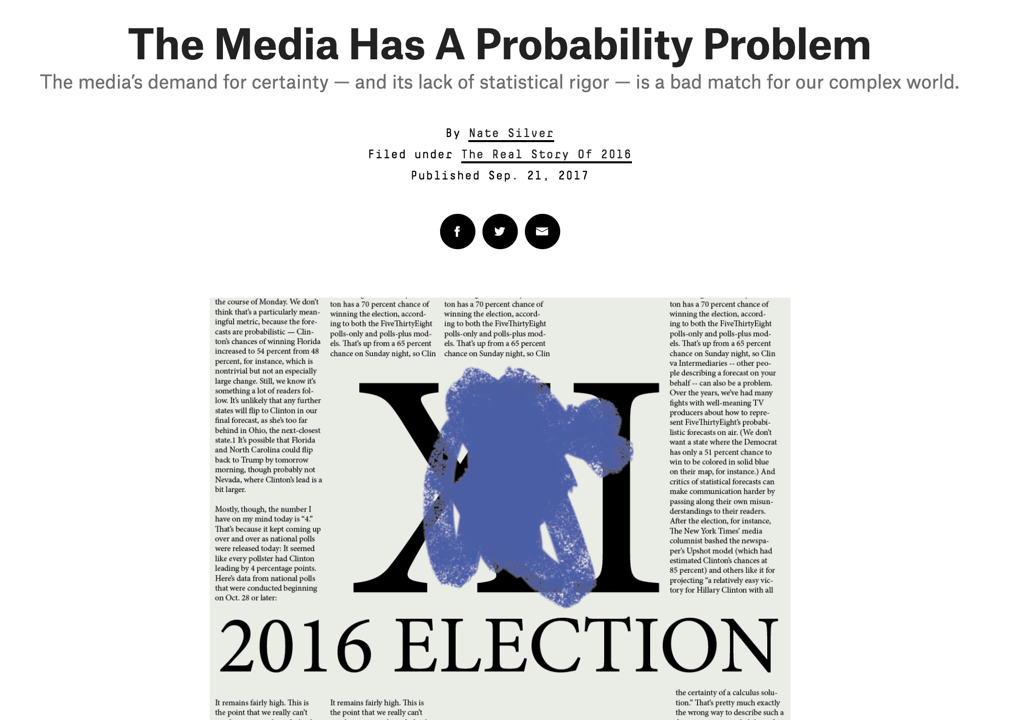
\includegraphics[width=8cm]{/Users/florianhollenbach/Documents/GitHub/Polisci209_2018/slides/week9/media_prob.png}
\end{center}
\end{frame}

\begin{frame}[label={sec:org0c4c1be}]{Why probability?}
\begin{itemize}
\item What are the chances it rains tomorrow?
\end{itemize}

\pause

\begin{itemize}
\item What are the chances you win the lottery?
\end{itemize}

\pause

\begin{itemize}
\item What is the probabilty of getting an A in pols 209?
\end{itemize}
\end{frame}

\begin{frame}[label={sec:org537c309}]{Why probability?}
\begin{itemize}
\item We use probability to express and calculate uncertainty

\item \emph{Preview}: later we will use probability to make statements about the uncertainty in our data analysis
\end{itemize}
\end{frame}

\begin{frame}[label={sec:org9b6750d}]{Two fundamental concepts of probability}
\begin{itemize}
\item Frequentist: long-run frequency of events
\begin{itemize}
\item \alert{ratio between the number of times the event occurs and the number of trials}
\item example: coin flips
\end{itemize}
\end{itemize}

\pause

\begin{itemize}
\item Bayesian: belief about the likelihood of event occurrence
\begin{itemize}
\item evidence based belief
\item often more sensible philosophy in political world
\end{itemize}
\end{itemize}
\end{frame}

\begin{frame}[label={sec:orgde47e32}]{Important Terms}
\begin{enumerate}
\item \alert{Experiment}: an action or a set of actions that produce stochastic events of interest
\end{enumerate}

\pause

\begin{enumerate}
\item \alert{sample space}: a set of all possible outcomes of the experiment, typically denoted by \(\Omega\)
\end{enumerate}

\pause

\begin{enumerate}
\item \alert{event}: a subset of the sample space
\end{enumerate}

(Imai - QSS)
\end{frame}

\begin{frame}[label={sec:orgb5c39d6}]{Example}
What is the experiment, sample space, and one event for coin flips or the pulling a single card out of a deck of 52?
\end{frame}

\begin{frame}[label={sec:org293ac4c}]{Defining Probability}
Probability of event A = P(A) = \(\frac{\text{number of elements in A}}{\text{number of elements in sample space}}\)

\pause

Probability of Head = P(H) = \(\frac{1}{2}\)
\end{frame}


\begin{frame}[label={sec:org05f8536}]{Example}
What is the probability of 3 head in 3 flips?

Sample space?

\pause

\(\Omega\) = \{HHH,HHT,HTH,THH, HTT, THT, TTH, TTT\}

\pause

What is the event space we are interested in?

\pause

\{HHH\}
\end{frame}

\begin{frame}[label={sec:org42e259d}]{Example}
What is the probability of 3 head in 3 flips?


\pause

P(HHH) = \(\frac{1}{8}\)
\end{frame}


\begin{frame}[label={sec:orgc2d41e8}]{Example}
What is the probability of 2 head in 3 flips?

\(\Omega\) = \{HHH,HHT,HTH,THH, HTT, THT, TTH, TTT\}

What is the event space we are interested in?

\pause

\{HHT, HTH, THH\}

\pause

P(2 H) = \(\frac{3}{8}\)
\end{frame}

\begin{frame}[label={sec:orgf110648}]{Axioms (rules) of Probability}
\begin{itemize}
\item the probability of \alert{any} event A is at least 0
\begin{itemize}
\item P(A) \(\geq\) 0
\end{itemize}
\end{itemize}

\pause

\begin{itemize}
\item The total sum of all possible outcomes in the sample space must be 1
\begin{itemize}
\item P(\(\Omega\)) = 1
\end{itemize}
\end{itemize}

\pause

\begin{itemize}
\item If A and B are mutually exclusive (\alert{meaning only one or the other can happen}), then P(A or B) = P(A) + P(B)
\end{itemize}
\end{frame}


\begin{frame}[label={sec:org3dd4cf2}]{Axioms (rules) of Probability}
A\(^{\text{c}}\) - complement to A, i.e. part of sample space not in A

Sometimes it is easier to calculate the probability of an event by using its complement
\end{frame}



\begin{frame}[label={sec:org49243e3}]{Using the complement:}
What is the probability of having at least one Tail on three coin flips?

\(\Omega\) = \{HHH,HHT,HTH,THH, HTT, THT, TTH, TTT\}

\pause

P(at least one T) = \(\frac{7}{8}\)

P(at least one T) = 1 - P(HHH) = 1 - \(\frac{1}{8}\)
\end{frame}



\begin{frame}[label={sec:org0a627ab}]{Example of simple probability}
What is the probability of getting a Queen as the first card from a full deck?

\(\Omega\) = \{?\}

Event space = \{?\}


\pause

p(Queen) = \(\frac{4}{52} = \frac{1}{13}\)
\end{frame}




\begin{frame}[label={sec:org8108ed4}]{How to quickly count the sample space when order matters: permutations}
\begin{itemize}
\item Often we do not want to or can't write out all possible combinations by hand

\item How many possibilities are there to arrange letters numbers 1,2,3?
\end{itemize}

\pause

Three outcomes: 1, 2, 3 \& three draws

\pause
First draw: A,B, or C

Second draw: two possibilities

Third draw: one left

3 x 2 x 1 possibilities
\end{frame}

\begin{frame}[label={sec:orgd9b1777}]{How to quickly count the sample space when order matters: permutations}
Permutations count many ways we can \alert{order} k objects out of a set of n unique objects

\(_{n}P_{k} = n \times (n-1) \times (n-2) \times ... \times (n-k + 1) = \frac{n!}{(n-k)!}\)

What does n! stand for?

\pause

n! = n-factorial = \$n \texttimes{} (n-1) \texttimes{} (n-2) \texttimes{} \ldots{} \texttimes{} (n-n+1)

\(3! = 3 \times 2 \times 1\)

\alert{Note: 0! = 1}
\end{frame}


\begin{frame}[label={sec:org424f11f}]{Permutation Example:}
How many ways can we arrange four cards out of a the 13 spades in our card deck?

first draw: ?
\pause

\(13 \times 12 \times 11 \times 10\)

\pause

\$ \frac{13!}{(13-4)!} =  \frac{13!}{9!} = 17160\$
\end{frame}

\begin{frame}[label={sec:orgd1d72f6}]{Birthday Problem}
Impress your family over Thanksgiving!

What is the probability that at least two people in this room have the same birthday?
\end{frame}


\begin{frame}[label={sec:orgb8ef819}]{Birthday Problem}
Can the law of total probabilities and complement help us?

\pause

Yes, P(at least two share bday) = 1 - P(nobody shares bday)
\end{frame}

\begin{frame}[label={sec:org06ba84d}]{Birthday Problem}
P(nobody shares bday)?

First find event space, i.e. everyone has a unique birthday

\pause

How many possibilities for birthdays in a year?

\pause

365

\pause

How many unique arrangements would we need for nobody to share the birthday?

\emph{number of people in room - k}
\end{frame}

\begin{frame}[label={sec:orgac1e74a}]{Birthday Problem}
\begin{enumerate}
\item \(_{365}P_{k} = \frac{365!}{(365-k)!}\) possibilities to arrange k unique birthdays over 365 days

\item What is the sample space? \alert{All the different possibilities for k birthdays (even non-unique).}
\end{enumerate}

\pause
\(365^{k}\)
\end{frame}

\begin{frame}[label={sec:org61c1cf3}]{Birthday Problem}
P(at least two share bday) = 1 - P(nobody shares bday) = 1 - \(\frac{365!}{(365-k)! \times 365^{k}}\)

\pause

P(at least two share bday): k = 10; 0.116, k = 23; 0.504, and k = 68; 0.999.
\end{frame}
\end{document}